%%%%%%%%%%%%%%%%%%%%%%%%%%%%%%%%%%%%%%%%%
% Large Colored Title Article
% LaTeX Template
% Version 1.1 (25/11/12)
%
% This template has been downloaded from:
% http://www.LaTeXTemplates.com
%
% Original author:
% Frits Wenneker (http://www.howtotex.com)
%
% License:
% CC BY-NC-SA 3.0 (http://creativecommons.org/licenses/by-nc-sa/3.0/)
%
%%%%%%%%%%%%%%%%%%%%%%%%%%%%%%%%%%%%%%%%%

%----------------------------------------------------------------------------------------
%	PACKAGES AND OTHER DOCUMENT CONFIGURATIONS
%----------------------------------------------------------------------------------------

\documentclass[DIV=calc, paper=a4, fontsize=11pt, twocolumn]{scrartcl}	 % A4 paper and 11pt font size

\usepackage{lipsum} % Used for inserting dummy 'Lorem ipsum' text into the template
\usepackage[english]{babel} % English language/hyphenation
\usepackage[protrusion=true,expansion=true]{microtype} % Better typography
\usepackage{amsmath,amsfonts,amsthm} % Math packages
\usepackage[svgnames]{xcolor} % Enabling colors by their 'svgnames'
\usepackage[hang, small,labelfont=bf,up,textfont=it,up]{caption} % Custom captions under/above floats in tables or figures
\usepackage{booktabs} % Horizontal rules in tables
\usepackage{fix-cm}	 % Custom font sizes - used for the initial letter in the document
\usepackage{graphicx}
\usepackage{sectsty} % Enables custom section titles
\allsectionsfont{\usefont{OT1}{phv}{b}{n}} % Change the font of all section commands

\usepackage{fancyhdr} % Needed to define custom headers/footers
\pagestyle{fancy} % Enables the custom headers/footers
\usepackage{lastpage} % Used to determine the number of pages in the document (for "Page X of Total")
\usepackage{caption}
\usepackage[font=small,labelfont=bf]{caption}

% Headers - all currently empty
\lhead{}
\chead{}
\rhead{}

% Footers
\lfoot{}
\cfoot{}
\rfoot{\footnotesize Page \thepage\ of \pageref{LastPage}} % "Page 1 of 2"

\renewcommand{\headrulewidth}{0.0pt} % No header rule
\renewcommand{\footrulewidth}{0.4pt} % Thin footer rule

\usepackage{lettrine} % Package to accentuate the first letter of the text
\newcommand{\initial}[1]{ % Defines the command and style for the first letter
\lettrine[lines=3,lhang=0.3,nindent=0em]{
\color{DarkGoldenrod}
{\textsf{#1}}}{}}

%----------------------------------------------------------------------------------------
%	TITLE SECTION
%----------------------------------------------------------------------------------------

\usepackage{titling} % Allows custom title configuration

\newcommand{\HorRule}{\color{DarkGoldenrod} \rule{\linewidth}{1pt}} % Defines the gold horizontal rule around the title

\pretitle{\vspace{-30pt} \begin{flushleft} \HorRule \fontsize{50}{50} \usefont{OT1}{phv}{b}{n} \color{DarkRed} \selectfont} % Horizontal rule before the title

\title{CCS Phase 1/2 Status Memo} % Your article title

\posttitle{\par\end{flushleft}\vskip 0.5em} % Whitespace under the title

\preauthor{\begin{flushleft}\large \lineskip 0.5em \usefont{OT1}{phv}{b}{sl} \color{DarkRed}} % Author font configuration

\author{ } % Your name

\postauthor{\footnotesize \usefont{OT1}{phv}{m}{sl} \color{Black} % Configuration for the institution name
% Your institution

\par
\end{flushleft}
\HorRule} % Horizontal rule after the title

\date{} % Add a date here if you would like one to appear underneath the title block

%----------------------------------------------------------------------------------------

\begin{document}

\maketitle % Print the title

\thispagestyle{fancy} % Enabling the custom headers/footers for the first page 

%----------------------------------------------------------------------------------------
%	ABSTRACT
%----------------------------------------------------------------------------------------

% The first character should be within \initial{}
\textbf{Although we are still in the process of evaluating how a Phase 2 model would perform for consensus calling by evaluating empirical error rates, this memo attempts to take an early look at how we may expect Phase 2 to perform on the Indel problem, and provide early insight into some challenges we may encounter.  My current sense is that the model will be good at predicting which bases should not be included, but less accurate at predicting when it needs to insert a base in a homopolymer context.  The assumption remains that it will beat the current approach at $>$10X.}

%----------------------------------------------------------------------------------------
%	ARTICLE CONTENTS
%----------------------------------------------------------------------------------------

\section*{Phase 1 Summary}

We trained a Phase 1 model on data derived from the  \texttt{ALL4MERS} template.  Using those parameters we evaluated how well they would call consensus sequences on a cross-validation set of ALL4MERs data from the same chip and run used for training.  The Phase 1 model used trains parameters for the $P(R|T)$ model.  In this model, the positions in the profile HMM are determined by the template, with the transition parameters into and out of each template position determined by the 4 channel SNRs and the  di-nucleotide contexts of the template positions.

On the cross-validated \texttt{ALL4MERS} data the Phase 1 model appeared to perform phenomenally well as shown in Figure 1.  Closer inspection showed that it did this by removing the systematic deletion errors in G/C homopolymers.

\begin{figure}[h]
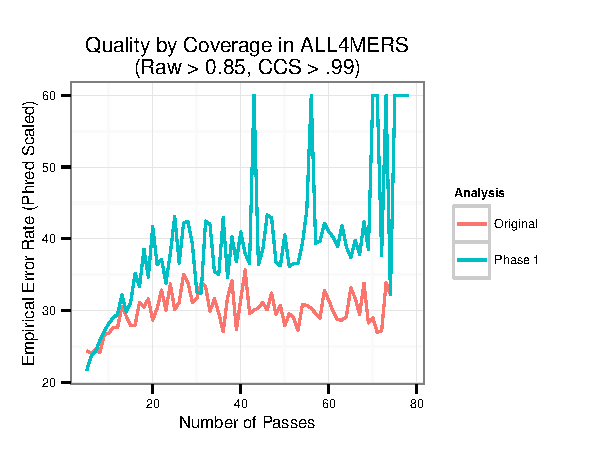
\includegraphics[width=\linewidth]{ALL4MERsErrorsWithCoverage}
\caption{Quality by coverage comparison for the ALL4MERS data.}
\end{figure}

A similar result was obtained for the HP template.  However, when the same model was applied to call consensus in $\lambda$ data from a different chip, the results were nowhere near as good.  Although the Phase 1 model again appeared to be asymptotically better, the cross over point was much further out and the low coverage accuracy was absolutely miserable (see figure 2).  

\begin{figure}[ht]
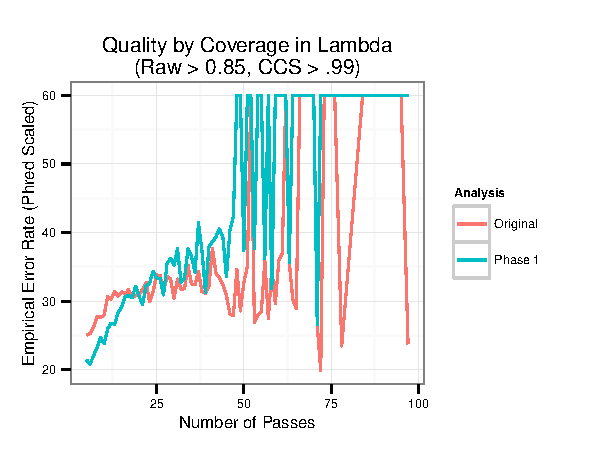
\includegraphics[width=\linewidth]{LambdaerrorsWithCoverage}
\caption{Quality by coverage comparison for the Lambda data.}
\end{figure}

Further examination showed that although in the $\lambda$ data the deletion errors had been removed, these were exchanged for insertion errors (compare the blue and orange symbols in Figure 3).

Although it is entirely possible that training on data more similar to $\lambda$ could generate superior results, even in the ALL4MER and NOHP data our predominant error mode amongst the residual errors was insertions.  As our Insertion QV appears to be able to give a reasonably good predictor of the probability of an insertion, we immediately went to Phase 2 in the hope that its $P(T|R)$ model would outperform Phase 1.

\begin{figure*}[ht]
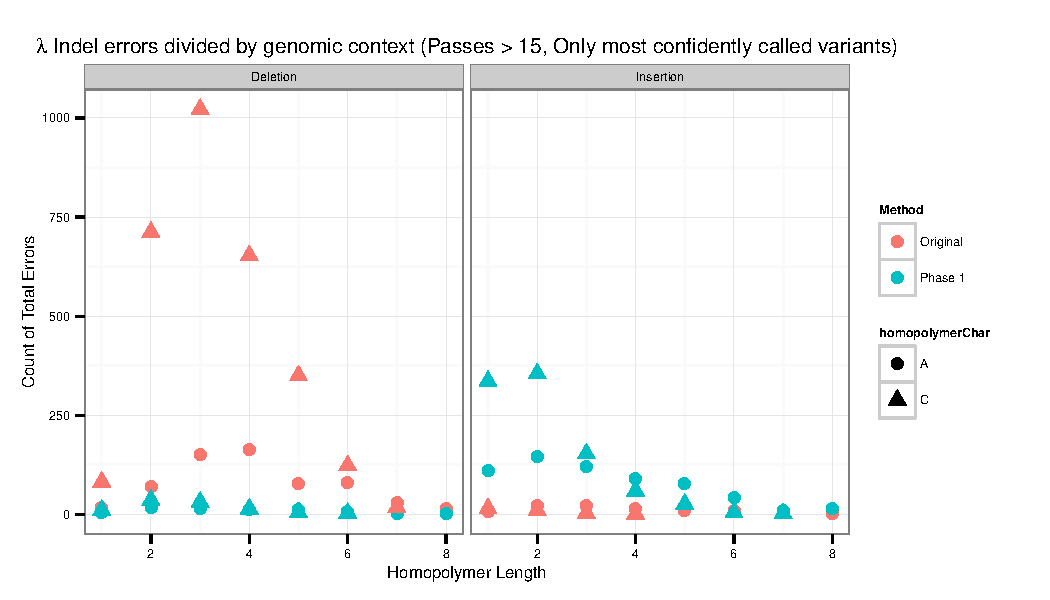
\includegraphics{LambdaByContext}
\caption{Indel errors by homopolymer context.}
\end{figure*}


%------------------------------------------------

\subsection*{Phase 2 and the Indel problem}

We have now fit the transition parameters for the Phase 2 model on $\lambda$ data and can evaluate certain characteristics about them.  Table 1 shows the Min/Max/Median and Mean of the transition parameters estimated for each read BP in our training data.  

\begin{table}[ht]
\caption{Phase 2 Transition Parameter Estimates}
\centering
\begin{tabular}{ | r | c | c | c | c | }
\hline

Statistic & Match & Stick & Branch & Deletion \\ \hline
Max & 0.99 & 0.44 & 0.66 & 0.86\\
Min & 0.11 & 4.89e-05 & 0.00156 & 0.002\\
Median & 0.94 & 0.012 & 0.01170 & 0.022\\ \hline
\textbf{Mean} & 0.88 & 0.021 & 0.023 & 0.076 \\
\bottomrule
\end{tabular}
\end{table}


The last row in this table, with the mean, can also be seen as giving the parameters for a ``constant" model where all the positions in a read are treated the same (As an aside, I think the 88\% mean match probability is the most interpretable number for our ``raw" accuracy).

This table shows a strong insertion bias in our read data, meaning consensus calls will have a strong deletion bias if the parameters are near the  ``constant" model.  From the perspective of the read, an insertion relative to the template corresponds to a deletion move through that read base, and the mean deletion move probability is $0.076 / 0.023 = 3.3$ times higher than the branch probability for that base.  As such, a simple model will prefer to remove read bases rather than add unobserved bases.

One effect of this probability difference can be seen by answer the following hypothetical question: Given a collection of reads from a 4 BP G homopolymer, what is the maximum percentage of 3 BP G reads (assuming only 4 bp and 3 bp reads exist) allowed before the incorrect sequence (3 BP) is called?

This number can be computed by assessing the likelihood for a 4 and 3 BP G homopolymer from each read type.  Table 2 shows the likelihood values for four read/template combinations.  We can see that a 3 bp read in the constant model votes with 3 likelihood units in favor of the 3 BP template, while the 4 BP read votes with 1.35 likelihood units against it.  By simple manipulations, this implies that if the 3 BP reads exceed 30\% of all the reads, the incorrect 3 bp HP will be called, which would be approximately as well as we do now, if not worse.

\begin{table}[ht]
\caption{Likelihood Values}
\centering
\begin{tabular}{ | l | l | c | c | }
\hline

Read & Template & LL & Difference \\ \hline
CCC & CCCC & -3.46 & -3.0 \\
CCC & CCC & -0.456 &   \\ \hline
CCCC & CCCC & -0.594 &1.35 \\
CCCC & CCC & -1.94 &   \\
\bottomrule
\end{tabular}
\end{table}

This would be unacceptably low accuracy, and the Phase 2 model will need to find co-variates that allow us to correctly identify sections of a read where a base should be removed, and other sections where it should be added, in order to overcome this bias and outperform the constant model.

Although how well the Phase 2 model will be able to correctly predict insertion and deletion events is ultimately an empirical question, in the next section we explore how the model seems to be doing at present.


%------------------------------------------------

\subsection*{Why so many insertions?}

At a high level, Pat decided that he wanted to have the base-caller be biased towards inserting bases, on the assumption that it would be easier to remove incorrect bases than add bases in.\footnote{See PulseToBaseStream.cs:571}  As a result, our consensus algorithms have a bias towards removing bases.

The hope in Phase 2 is that we can capture information that will allow us to ``disregard" incorrectly inserted bases, and also identify when bases need to be added in, particularly in homopolymer contexts.  Do we have such information?

One indication that the model is able to pick up on useful information is the distribution of estimated transition probabilities for different read bases, as shown in Figure 4.  Here we see that values range quite widely, particularly for the Deletion move (corresponding to removing an incorrectly inserted base from the read).  As an example of the desired behavior, if in our 4 BP G homopolymer example, if all of the 4 BP reads had low Deletion transition probabilities, and all the 3 BP read had high Branch probabilities, we will definitely outperform the constant rate model.

\begin{figure*}[ht]
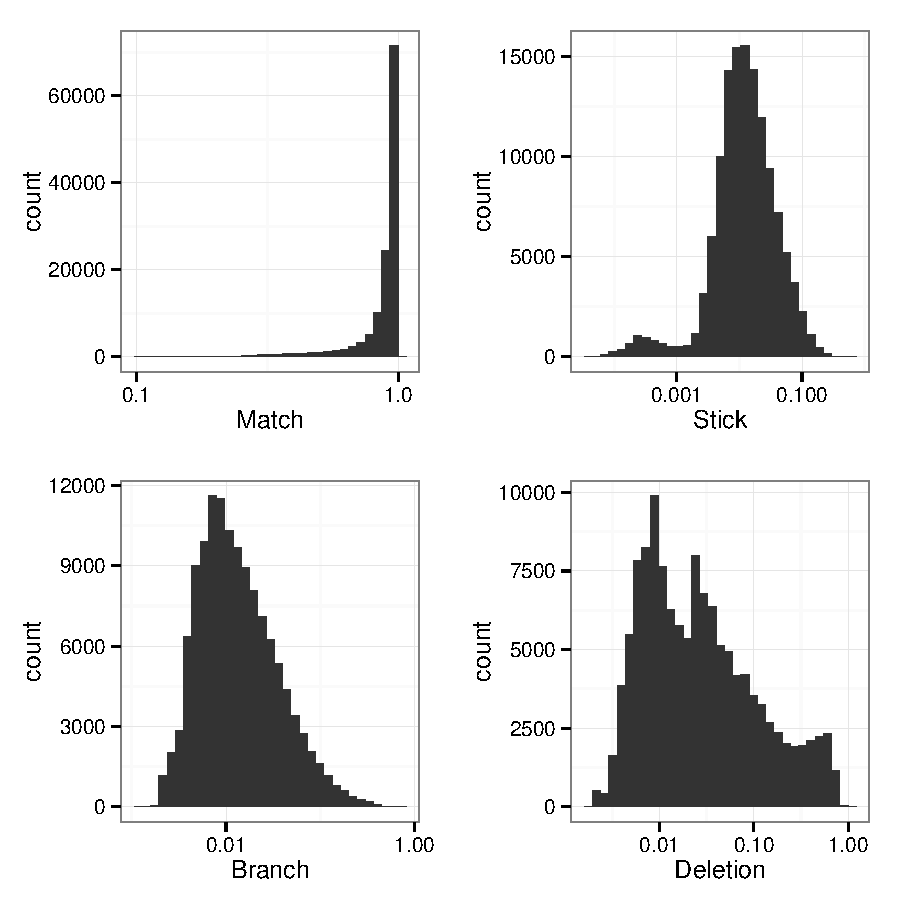
\includegraphics{ParameterDistributions}
\caption{Histogram of Marginal Transition Parameters}
\end{figure*}


\subsection*{How QVs relate to Indel Probabilities}

The linear modeling showed that one of the largest drops in AIC could be obtained by simply adding the Insertion QV into the model.  An examination of how this parameter is used by the model to make predictions shows that the model can identify when a read base should be deleted (Figure 5).  For this reason, we are optimistic that Phase 2 may be able to remove several of the size 1 insertion errors seen in Phase 1.

\begin{figure}[ht]
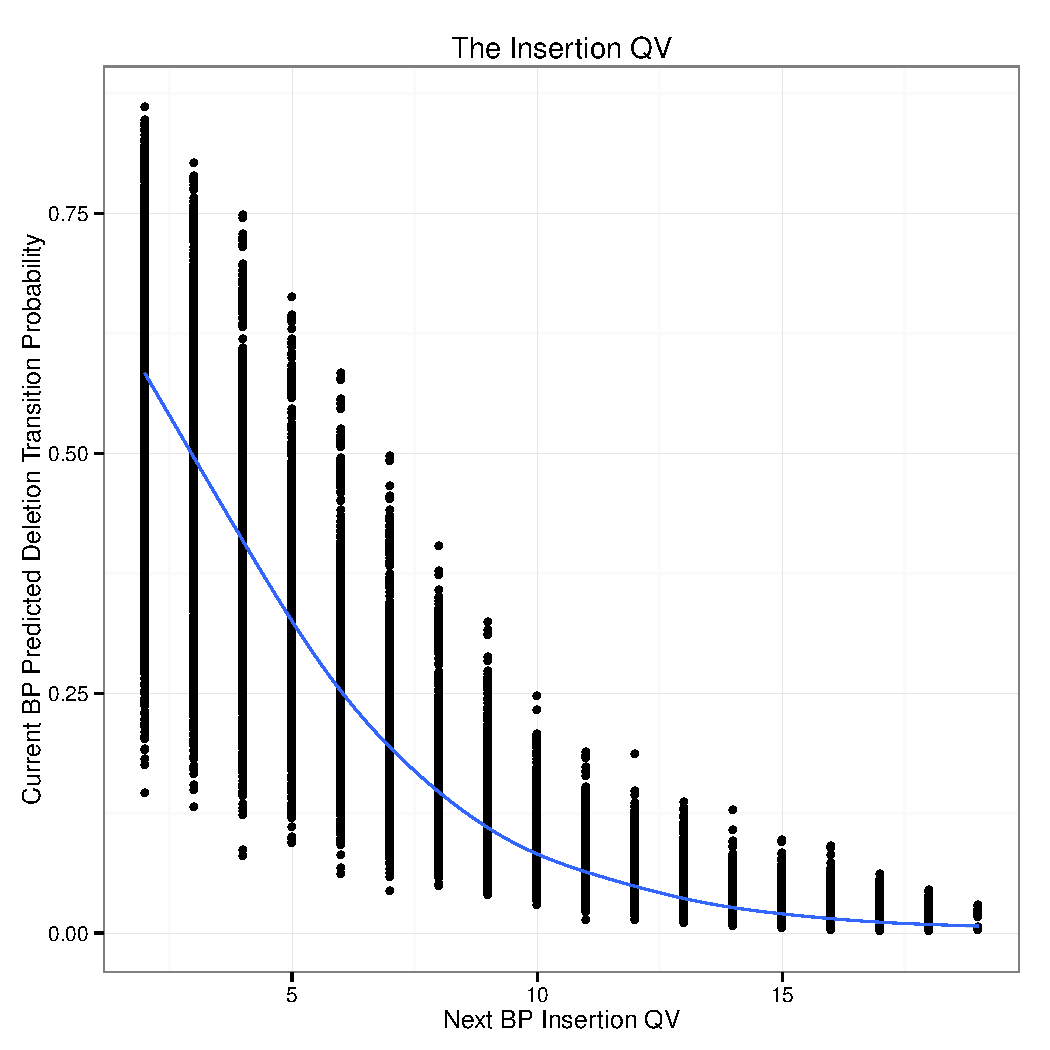
\includegraphics[width=\linewidth]{IQV}
\caption{How IQV effects the prediction of an Insertion.}
\end{figure}

The other half of the equation though is predicting when a base should be placed in a read but was not (e.g. $\texttt{GGG} \rightarrow \texttt{GGGG}$).  Although simply refining the deletion probabilities may be enough to get us to our accuracy objective, we do not at present appear to generate predictions of the Branch rate that are nearly as variable as our Deletion predictions.  Figure 6 shows the predicted Branch rate versus the Posterior Expectation (Pseudo-counts) for each site.  Unfortunately, 95\% of our Branch transition rate predictions are 0.08\% probability or less, and in general there is little variation in the predicted Branch probability.  In contrast, in the Phase 1 model we estimated that on average $CC$ can be emitted as $C$ approximately 22\% of the time at low SNR, and saw quite a bit of variation across SNR.  It would be nice if we could get similar variability for our Branch predictions, and future efforts will go towards this.

\begin{figure*}[ht]
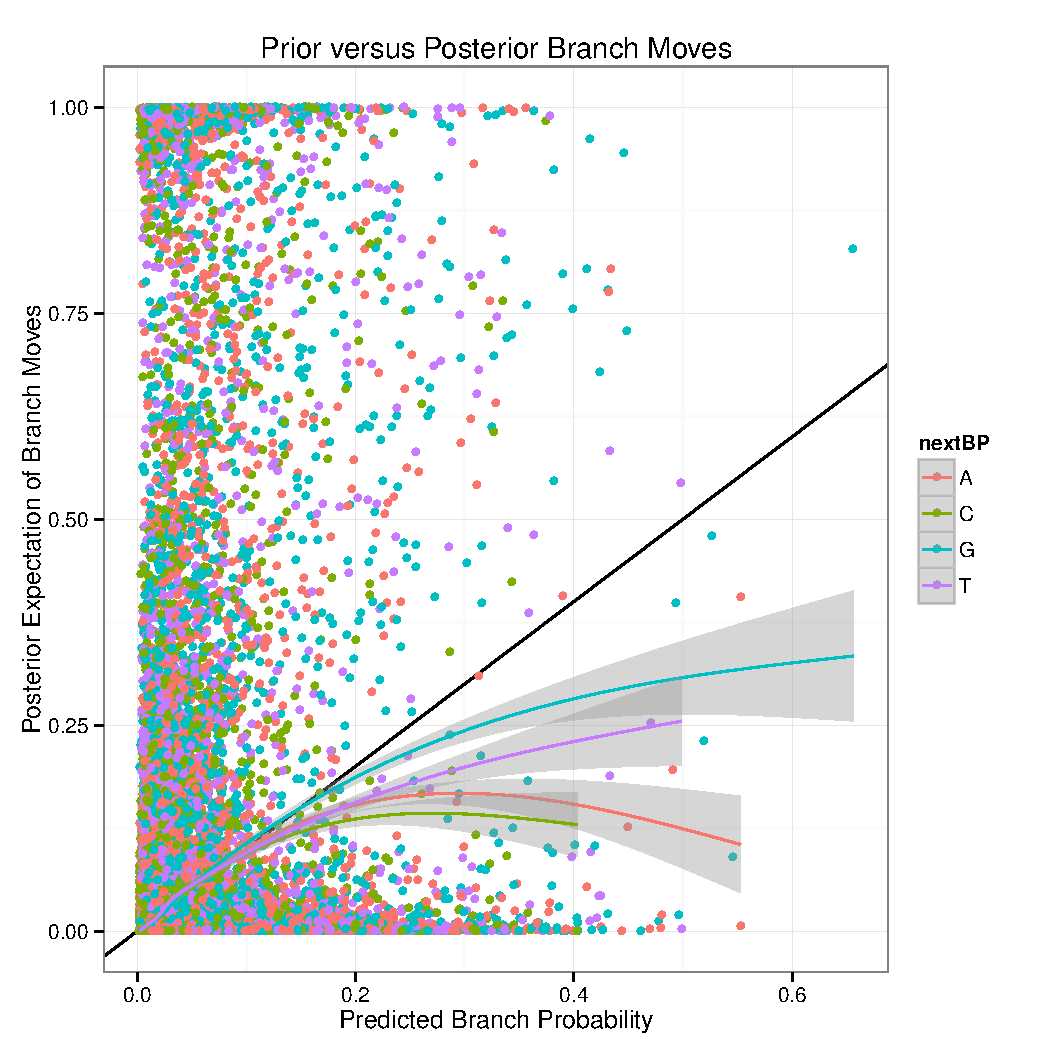
\includegraphics[width=\linewidth]{BranchMoves}
\caption{Branch Rate Prediction Qualities}
\end{figure*}


\

\end{document}